\hypertarget{burstiness}{%
\subsubsection{Burstiness}\label{burstiness}}

Question: How are short timeframes of intense activity, followed by a
corresponding return to a typical pattern of activity, observed in a
project?

\hypertarget{description}{%
\paragraph{Description}\label{description}}

There are a number of reasons that may prompt a sudden increase or
decrease in the amount of activity within a repository. These increases
and decreases appear both as a sudden change in activity against the
average amount of activity. Burstiness is a way of understanding the
cycle of activity in existing metrics, like issues, merge requests,
mailing lists, commits, or comments. Examples of root causes for bursts
in activity include:

\begin{itemize}
\tightlist
\item
  Release cycles
\item
  Global pandemics
\item
  Hackathon activities
\item
  Mentorship programs
\item
  Conferences, meetups, and other events where tools are presented
\item
  Conventional and social media announcements and mentions
\item
  Critical bugs as raising awareness and getting people's attention
\item
  Community design meetings or brainstorming meetings to address a
  particular issue
\item
  Community members show up from another community that is relying on
  your project (e.g., dependencies)
\end{itemize}

\hypertarget{objectives}{%
\paragraph{Objectives}\label{objectives}}

\begin{itemize}
\tightlist
\item
  To identify impacts of root causes of a burst in activity
\item
  To provide awareness when project activity unknowingly goes up
\item
  To help capture the meaningfulness of increases or decreases in
  project activity
\item
  To help the community and maintainers prepare for future bursts that
  follow a pattern
\item
  To help measure the impact of influential external activities
\item
  To differentiate skewed activity versus normal activity
\end{itemize}

\hypertarget{implementation}{%
\paragraph{Implementation}\label{implementation}}

\hypertarget{filters}{%
\subparagraph{Filters}\label{filters}}

\begin{itemize}
\tightlist
\item
  Stars
\item
  Forks
\item
  Issues or bug reports
\item
  Labels
\item
  Downloads
\item
  Release Tags
\item
  Change Requests
\item
  Mail List Traffic
\item
  Documentation additions or revisions
\item
  New Repositories
\item
  Feature Requests
\item
  Messaging Conversations
\item
  Conventional and Social Media Activity
\item
  Conference Attendance and Submissions
\end{itemize}

\hypertarget{visualizations}{%
\subparagraph{Visualizations}\label{visualizations}}

Augur:

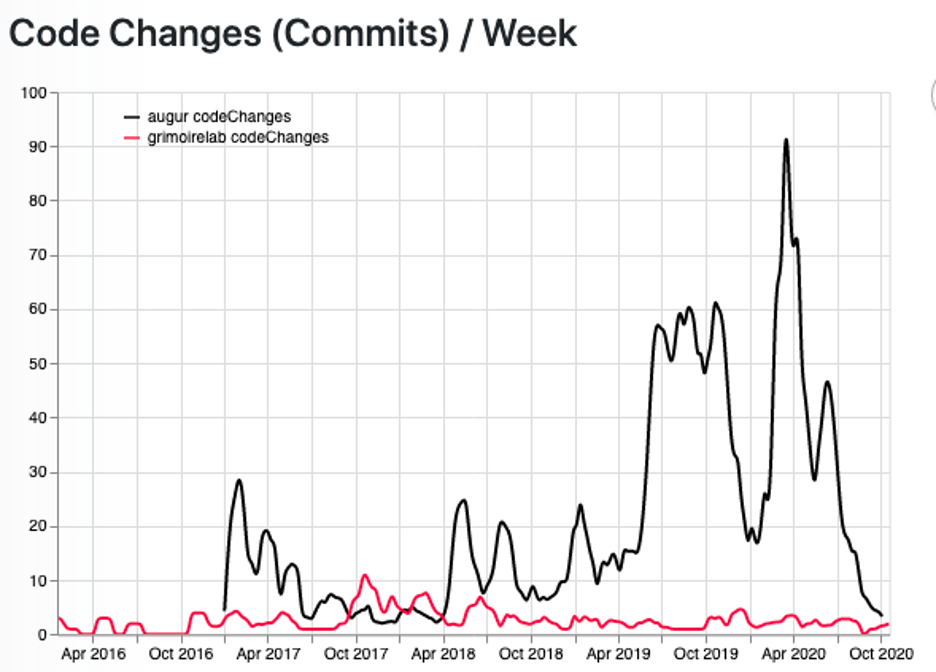
\includegraphics{images/burstiness_augur.png}

GrimoireLab:

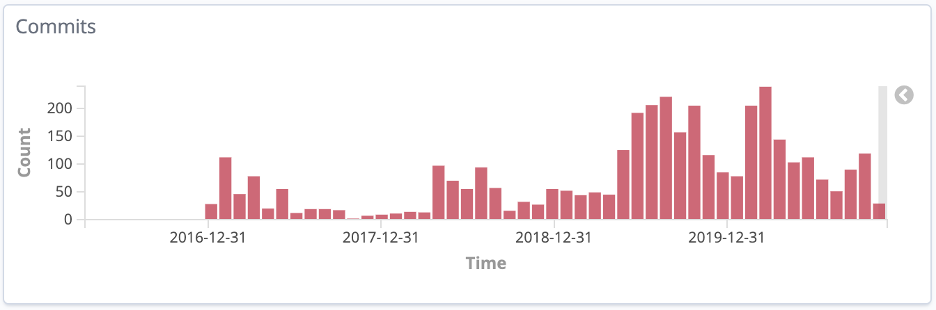
\includegraphics{images/burstiness_gl.png}

\hypertarget{tools-providing-the-metric}{%
\subparagraph{Tools Providing the
Metric}\label{tools-providing-the-metric}}

\begin{itemize}
\tightlist
\item
  Grimoire Lab
\item
  Augur
\end{itemize}

\hypertarget{data-collection-strategies}{%
\subparagraph{Data Collection
Strategies}\label{data-collection-strategies}}

\begin{itemize}
\item
  Quantitative

  \begin{itemize}
  \tightlist
  \item
    Time box activities identifying deviations away from some norm
  \item
    Outliers for certain thresholds, using statistics like Bollinger
    Bands to measure stability or volatility:
    \href{https://en.wikipedia.org/wiki/Bollinger_Bands}{https://en.wikipedia.org/wiki/Bollinger\_Bands}
  \end{itemize}
\item
  Qualitative Interview Questions

  \begin{itemize}
  \tightlist
  \item
    Why do you contribute more during a period of time?
  \item
    What do you believe to be the root cause for particular bursts?
  \item
    What impact do different events (e.g., hackathons, mentorship
    program, or conferences) have on project activity?
  \end{itemize}
\end{itemize}

\hypertarget{references}{%
\paragraph{References}\label{references}}

This metric was inspired by the work of Goh and Barabasi (2008):
\href{https://arxiv.org/pdf/physics/0610233.pdf}{https://arxiv.org/pdf/physics/0610233.pdf}
